\documentclass[12pt,oneside, a4j]{jbook}
%
\usepackage{amsmath}%,amssymb}
\usepackage{txfonts}
\usepackage[dvipdfmx]{graphicx}
\usepackage{booktabs}
\usepackage{enumerate}
\usepackage{cite}
\usepackage{url}
%\usepackage{wrapfig}
%\usepackage{ascmac}
%\usepackage{makeidx}
%\usepackage{bm}
%\usepackage{subfigure}
%\usepackage{verbatim}
%
%\setlength{\textwidth}{\fullwidth}
%\addtolength{\textheight}{\topskip}
%%Math
%\newcommand{\diff}{\mathrm{d}}  %微分記号
%\newcommand{\divergence}{\mathrm{div}\,}  %ダイバージェンス
%\newcommand{\grad}{\mathrm{grad}\,}  %グラディエント
%\newcommand{\rot}{\mathrm{rot}\,}  %ローテーション

\begin{document}
\frontmatter
%Title
\title{東海大学大学院 2016年 修士論文 \\\\\\ \\ \\ ハイブリッドロケット液体酸素\\気化に関する研究}
\author{\\ \\ \\指導教員:\\\\\\東海大学大学院工学研究科\\航空宇宙学専攻\\\\\\学生番号:4bmjm020 三島源生}
\maketitle

\chapter*{概要}
\ 
考え中
\\


\tableofcontents
\listoftables
\listoffigures

\clearpage

\mainmatter
\chapter{序論}
本章では、まず研究の背景として、現在のロケット業界とハイブリッドロケットとの関係性について説明する。

\section{研究背景}
%\subsection{研究背景}
近年宇宙産業は新興国も含めて世界中で需要が拡大しており、
アメリカの調査会社は超小型衛星(1-50kg)需要が2020年までに400−500機ほどになると予想している。\cite{nano/micro}
我が国においても新たな産業需要を見込んでおり、
従来の通信・放送に加え、災害監視・環境観測・農林漁業・国土監視・資源探査・安全保障などの地球観測の分野での利用拡大が予想されている。
その一方で宇宙輸送技術は発展途上段階にあり非常に高価なものである。
現在打ち上げられている超小型衛星の90\%は大型衛星に相乗りして打ち上げられたものであり、
打ち上げ機会また条件が限られているため、
この超小型衛星の需要を満たすことができないと予想されている。

%\subsection{ハイブリッドロケット}
ハイブリッドロケットは科学推進ロケットの一つである。
科学推進ロケットは推進剤の酸化剤と燃料を燃焼させることで生じる高温・高圧の燃焼ガスをノズルにより膨張させることで、高速噴流を作り、推力を得るロケットである。
燃焼形態は予混合燃焼と拡散燃焼に分類することができ、


近年宇宙産業は新興国も含めて世界中で需要が拡大しており、
アメリカの調査会社は超小型衛星(1-50kg)需要が2020年までに400−500機ほどになると予想している。\cite{nano/micro}
我が国においても新たな産業需要を見込んでおり、
従来の通信・放送に加え、災害監視・環境観測・農林漁業・国土監視・資源探査・安全保障などの地球観測の分野での利用拡大が予想されている。
その一方で宇宙輸送技術は発展途上段階にあり非常に高価なものである。
現在打ち上げられている超小型衛星の90\%は大型衛星に相乗りして打ち上げられたものであり、
打ち上げコストが高くまた機会・条件が限られているため、
超小型衛星の需要を満たす宇宙輸送機を供給することができないと予想されている。
この供給量を増やすためには以下のコスト削減手段が考えられる。
\begin{itemize}
	\item 生産性と効率の改善
	\begin{itemize}
		\item 各構成要素の規格化と一般化
		\item 量産システムの構築
	\end{itemize}
	\item 商業化・自由競争による促進
	\item 技術的なイノベーション
	\begin{itemize}
		\item 再使用ロケット
		\item 3-Dプリンターによる製造
		\item ロケットの潜在的危険性を取り除いた設計 (Delethalizing)
	\end{itemize}
\end{itemize}
過去25年間(1980年-2004年)における世界の宇宙機打ち上げの調査により、打ち上げ失敗は推進システムによるものが優位を占めていることがわかっている。\cite{failure}

ハイブリッドロケットは科学推進ロケットの一つである。
科学推進ロケットは推進剤の酸化剤と燃料を燃焼させることで生じる高温・高圧の燃焼ガスをノズルにより膨張させることで、高速噴流を作り、推力を得るロケットである。
燃焼形態は予混合燃焼と拡散燃焼に分類することができ、


\section{実験装置}
\subsection{供試体}
本実験では2種類の供試体を使用した。
液体酸素はインジェクタを通して供試体に流入する。燃料のあるプリバーナ部で燃焼をさせ、バッフルプレートを通して混合室部に流入しノズルから気体酸素と燃焼ガスが排出される。ノズルより下流は大気圧となっている。気化器の概略図を図\ref{fig:PBOut}に示す。
インジェクタには$\phi$0.3mmの孔が20個ある。それぞれの位置は軸中心から$\phi$12mmの位置に位相45°で8孔、$\phi$24mmの位置に位相30°で12孔とした。インジェクタ外観を図\ref{fig:Injector}に示す。
プリバーナ部の燃料の長さに応じてスペーサ(グラファイト)を詰めた。
供試体1は気化器内部の状態を可視化するために、プリバーナ部と混合室部の外殻にアクリル樹脂、混合室部の内壁に石英ガラスを使用した。
供試体2は基礎データ取得のために、プリバーナ部と混合室部の外殻にステンレスと混合室部の内壁にグラファイトを使用した。
プリバーナ部と混合室部を分けるバッフルプレートは$\phi$18mmの位置に孔を8孔開けた布ベークライト製のものと穴を4孔開けたグラファイト製のもの2種類を製作した。それぞれ穴の位相は45°と90°である。バッフルプレート外観を図\ref{Baffle}に示す。
ノズルは$\phi8.5mm$、グラファイトで製作した。
気化器1断面図を図\ref{fig:Chamber1},気化器2断面図を図\ref{fig:Chamber2}に示す。




\subsection{供給系}
本供給系は植松電機殿の設備を使用した。
供給系系統図を図\ref{fig:LOXLine}に示す。

%\begin{figure}[htbp]
%\begin{tabular}{cc}
%\begin{minipage}{.5\textwidth}
%\begin{center}
%\centering
%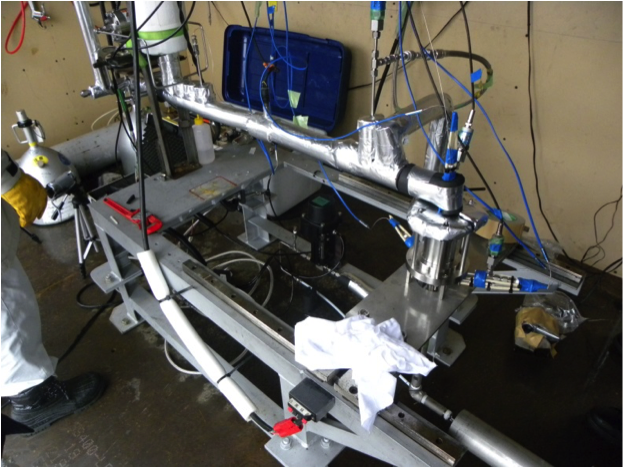
\includegraphics[width=7cm]{\FigAddTwo/LOXLinePho.png}
%\caption{LOXタンク外観}
%\label{fig:LOXTankPho}
%\end{center}
%\end{minipage}
%\begin{minipage}{.5\textwidth}
%\begin{center}
%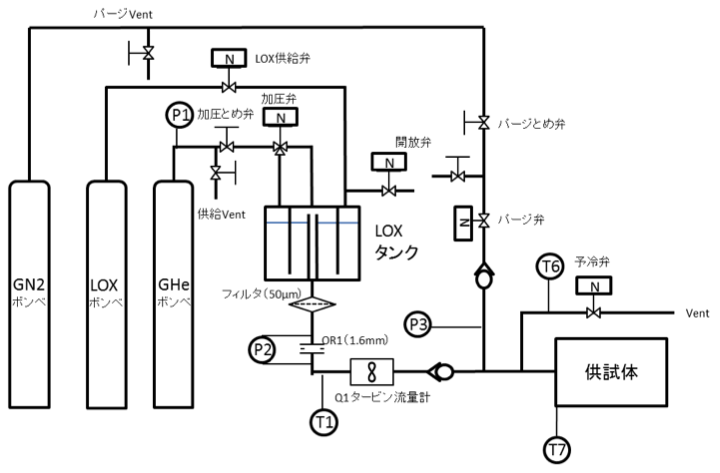
\includegraphics[width=7cm]{\FigAddTwo/LOXLine.png}
%\caption{LOX配管図}
%\end{center}
%\end{minipage}
%\end{tabular}
%\end{figure}

%\begin{figure}
%\centering
%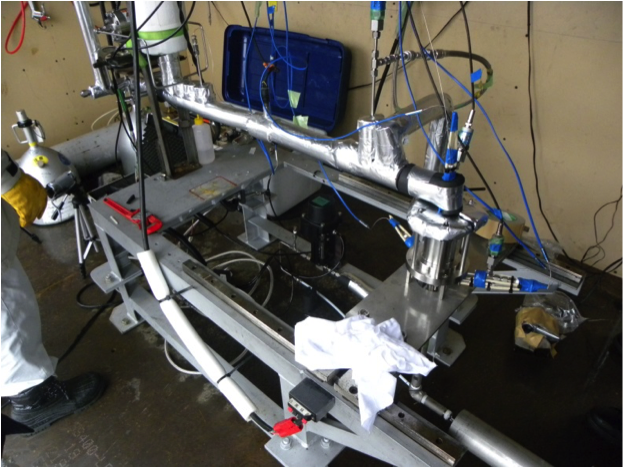
\includegraphics[width=15cm]{\FigAddTwo/LOXLinePho.png}
%\caption{LOXタンク外観}
%\label{fig:LOXTankPho}
%\end{figure}

\begin{figure}
\centering
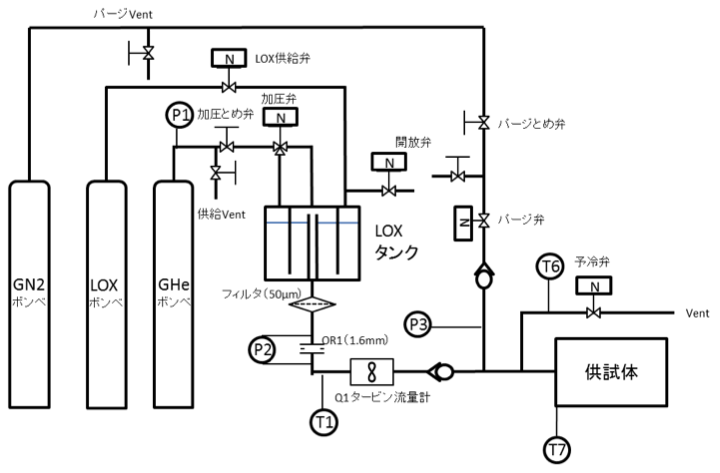
\includegraphics[width=15cm]{\FigAddTwo/LOXLine.png}
\caption{供給系系統図}
\label{fig:LOXLine}
\end{figure}

\subsection{計測系}
データロガーには、植松電機殿所有のEDX-100Aを用いた。サンプリングレートは200Hzとした。計測項目を以下に示す。
\begin{description}
\item[P1]GHe供給圧
\item[P2]オリフィス差圧
\item[P3]インジェクタ上流圧
\item[P4]プリバーナ圧
\item[P5]混合室圧
\item[Q1]LOX体積流量
\item[T1]オリフィス下流温度
\item[T2]インジェクタ上流温度
\item[T3]ノズル上流温度(内径)
\item[T4]ノズル上流温度(中心)
\item[T5]ノズル下流温度
\item[T6]予鈴温度
\item[T7]インジェクタフランジ温度
\end{description}
供試体周りの計測系の概略図を図\ref{}に、ノズル付近の内観を図\ref{fig:NozzleThermo}示す。
\\
高速度カメラによる可視化データ取得も行った。

\begin{figure}[htbp]
\begin{tabular}{cc}
\begin{minipage}{.5\textwidth}
\begin{center}
\centering
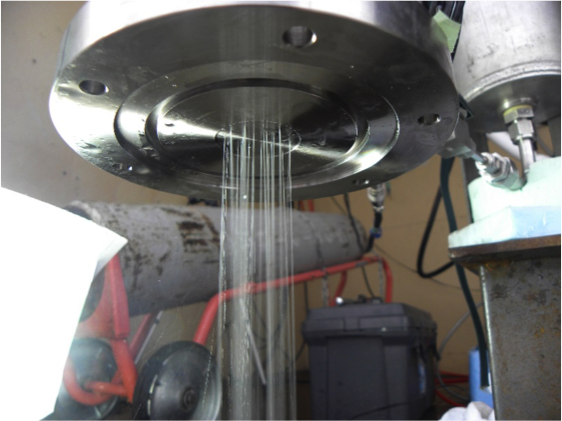
\includegraphics[width=7cm]{\FigAddTwo/Injector.png}
\caption{インジェクタ外観}
\label{fig:Injector}
\end{center}
\end{minipage}
\begin{minipage}{.5\textwidth}
\begin{center}
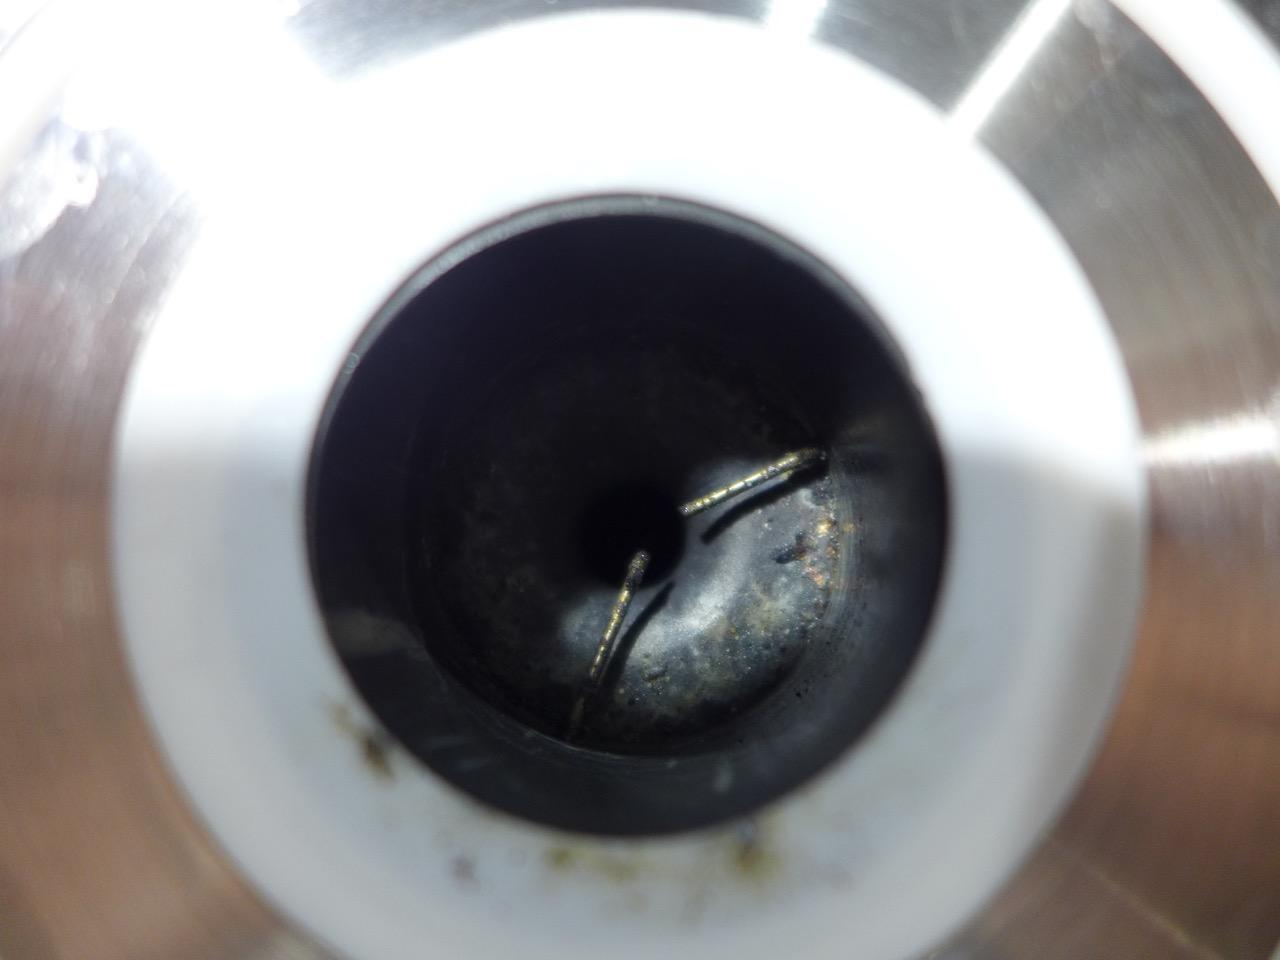
\includegraphics[width=7cm]{\FigAddTwo/NozzleThermo.jpg}
\caption{ノズル付近内観}
\label{fig:NozzleThermo}
\end{center}
\end{minipage}
\end{tabular}
\end{figure}

\subsection{制御系}
制御系は、植松電機どの所有の設備を用いた。ニクロム線加熱スイッチ、開放弁スイッチ、パージベンスイッチ、冷却弁スイッチにより構成されている。ニクロム線加熱時間、加圧弁開放時間、開放弁開はタイマーにより制御可能である。
\\
供試体1を使用した燃焼気化実験では、ニクロム線を加熱を開始した後に、LOXタンクの自己加圧によりインジェクタから放出される酸素と燃料が着火したことをビデオモニタにより確認した時に、加圧弁スイッチをオンにし、本着火を開始した。
規定の加圧弁開時間を終了したところで、加圧弁が閉じられて、開放弁が開となりLOXタンク圧力が開放される。それと同時に手動でパージ弁を開とし、窒素によるパージを行う。
供試体2を使用した燃焼気化実験では、外殻をステンレスで覆っているため、ノズル上流温度が上昇し始めたら着火したと判定し、加圧弁スイッチをオンにした。その他の手順は供試体1での実験と同様である。
ニクロム線設置位置を図\ref{fig:Nichrome}、着火判定した点を図\ref{fig:Ignition}
\begin{figure}
\centering
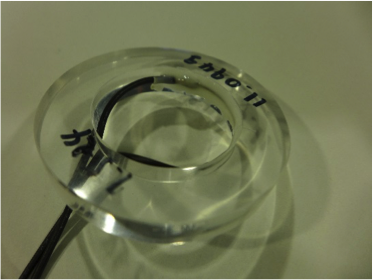
\includegraphics[width=10cm]{\FigAddTwo/Nichrome.png}
\caption{ニクロム線}
\label{fig:Nichrome}
\end{figure}
\begin{figure}
\centering
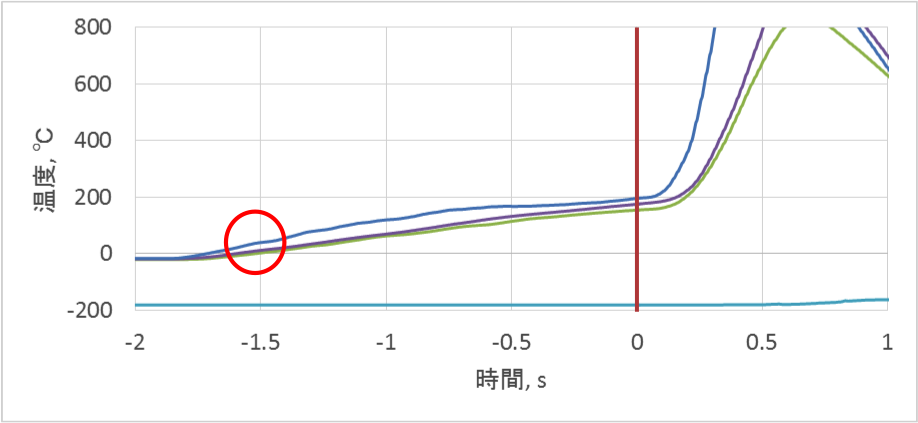
\includegraphics[width=11cm]{\FigAddTwo/Ignition.png}
\caption{着火判定した点}
\label{fig:Ignition}
\end{figure}



\section{水流し試験}
本実験では流量計測にタービン流量計の他にオリフィス差圧とインジェクタ差圧を使用した。
差圧から流量を計測するために、各差圧の流量係数を確認する必要がある。
GHe供給圧をパラメータとし、水を30秒以上流し、噴出した水の総量から、水の流量を求めた。水の噴射の様子を図に示す。
\\
流量定数はベルヌーイの定理と連続の式から導出できる。
\begin{eqnarray}
P_{1} + \frac{1}{2} \rho_{1} u^2_{1} &=& P_{2} + \frac{1}{2} \rho_{2} u^2_{2}  \nonumber \\
u^2_{2} - u^2_{1} &=& \frac{2(P_{1}-P_{2})}{\rho} 
\label{eq:vel}
\end{eqnarray}
\begin{eqnarray}
u_{1}A_{1} &=& u_{2}A_{2}  \nonumber \\
u_{2} &=& u_{1}\frac{A_{1}}{A_{2}}
\label{eq:con}
\end{eqnarray}
\ref{eq:con}を\ref{eq:vel}に代入する。
%\begin{eqnarray}
%u_{2}=\frac{1}{\sqrt{1-(\frac{A_2}{A_1})^2}} \sqrt{\frac{2(P_{1}-P_{2})}} \\
%\end{eqnarray}



\clearpage
\chapter{}
この章では実験手法と計測項目について説明する。

\section{研究背景}
%\subsection{研究背景}
近年宇宙産業は新興国も含めて世界中で需要が拡大しており、
アメリカの調査会社は超小型衛星(1-50kg)需要が2020年までに400−500機ほどになると予想している。\cite{nano/micro}
我が国においても新たな産業需要を見込んでおり、
従来の通信・放送に加え、災害監視・環境観測・農林漁業・国土監視・資源探査・安全保障などの地球観測の分野での利用拡大が予想されている。
その一方で宇宙輸送技術は発展途上段階にあり非常に高価なものである。
現在打ち上げられている超小型衛星の90\%は大型衛星に相乗りして打ち上げられたものであり、
打ち上げ機会また条件が限られているため、
この超小型衛星の需要を満たすことができないと予想されている。

%\subsection{ハイブリッドロケット}
ハイブリッドロケットは科学推進ロケットの一つである。
科学推進ロケットは推進剤の酸化剤と燃料を燃焼させることで生じる高温・高圧の燃焼ガスをノズルにより膨張させることで、高速噴流を作り、推力を得るロケットである。
燃焼形態は予混合燃焼と拡散燃焼に分類することができ、


近年宇宙産業は新興国も含めて世界中で需要が拡大しており、
アメリカの調査会社は超小型衛星(1-50kg)需要が2020年までに400−500機ほどになると予想している。\cite{nano/micro}
我が国においても新たな産業需要を見込んでおり、
従来の通信・放送に加え、災害監視・環境観測・農林漁業・国土監視・資源探査・安全保障などの地球観測の分野での利用拡大が予想されている。
その一方で宇宙輸送技術は発展途上段階にあり非常に高価なものである。
現在打ち上げられている超小型衛星の90\%は大型衛星に相乗りして打ち上げられたものであり、
打ち上げコストが高くまた機会・条件が限られているため、
超小型衛星の需要を満たす宇宙輸送機を供給することができないと予想されている。
この供給量を増やすためには以下のコスト削減手段が考えられる。
\begin{itemize}
	\item 生産性と効率の改善
	\begin{itemize}
		\item 各構成要素の規格化と一般化
		\item 量産システムの構築
	\end{itemize}
	\item 商業化・自由競争による促進
	\item 技術的なイノベーション
	\begin{itemize}
		\item 再使用ロケット
		\item 3-Dプリンターによる製造
		\item ロケットの潜在的危険性を取り除いた設計 (Delethalizing)
	\end{itemize}
\end{itemize}
過去25年間(1980年-2004年)における世界の宇宙機打ち上げの調査により、打ち上げ失敗は推進システムによるものが優位を占めていることがわかっている。\cite{failure}

ハイブリッドロケットは科学推進ロケットの一つである。
科学推進ロケットは推進剤の酸化剤と燃料を燃焼させることで生じる高温・高圧の燃焼ガスをノズルにより膨張させることで、高速噴流を作り、推力を得るロケットである。
燃焼形態は予混合燃焼と拡散燃焼に分類することができ、


\section{実験装置}
\subsection{供試体}
本実験では2種類の供試体を使用した。
液体酸素はインジェクタを通して供試体に流入する。燃料のあるプリバーナ部で燃焼をさせ、バッフルプレートを通して混合室部に流入しノズルから気体酸素と燃焼ガスが排出される。ノズルより下流は大気圧となっている。気化器の概略図を図\ref{fig:PBOut}に示す。
インジェクタには$\phi$0.3mmの孔が20個ある。それぞれの位置は軸中心から$\phi$12mmの位置に位相45°で8孔、$\phi$24mmの位置に位相30°で12孔とした。インジェクタ外観を図\ref{fig:Injector}に示す。
プリバーナ部の燃料の長さに応じてスペーサ(グラファイト)を詰めた。
供試体1は気化器内部の状態を可視化するために、プリバーナ部と混合室部の外殻にアクリル樹脂、混合室部の内壁に石英ガラスを使用した。
供試体2は基礎データ取得のために、プリバーナ部と混合室部の外殻にステンレスと混合室部の内壁にグラファイトを使用した。
プリバーナ部と混合室部を分けるバッフルプレートは$\phi$18mmの位置に孔を8孔開けた布ベークライト製のものと穴を4孔開けたグラファイト製のもの2種類を製作した。それぞれ穴の位相は45°と90°である。バッフルプレート外観を図\ref{Baffle}に示す。
ノズルは$\phi8.5mm$、グラファイトで製作した。
気化器1断面図を図\ref{fig:Chamber1},気化器2断面図を図\ref{fig:Chamber2}に示す。




\subsection{供給系}
本供給系は植松電機殿の設備を使用した。
供給系系統図を図\ref{fig:LOXLine}に示す。

%\begin{figure}[htbp]
%\begin{tabular}{cc}
%\begin{minipage}{.5\textwidth}
%\begin{center}
%\centering
%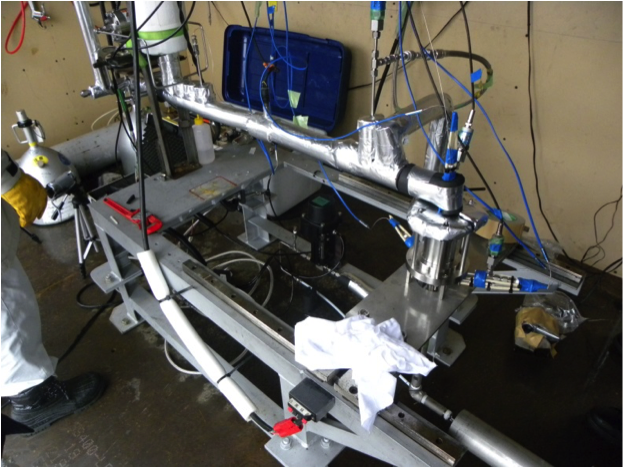
\includegraphics[width=7cm]{\FigAddTwo/LOXLinePho.png}
%\caption{LOXタンク外観}
%\label{fig:LOXTankPho}
%\end{center}
%\end{minipage}
%\begin{minipage}{.5\textwidth}
%\begin{center}
%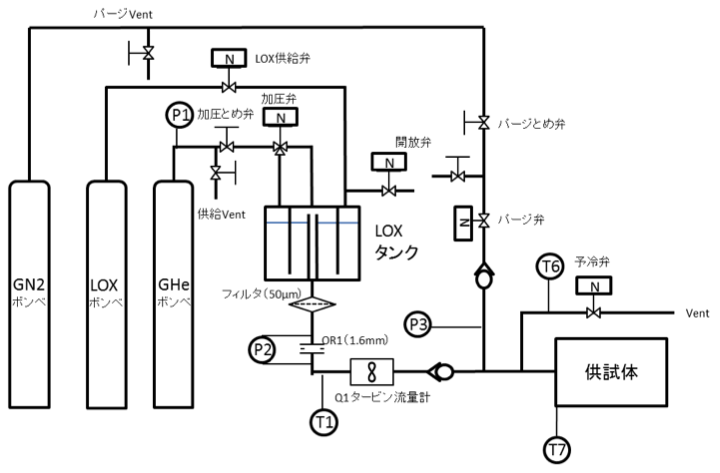
\includegraphics[width=7cm]{\FigAddTwo/LOXLine.png}
%\caption{LOX配管図}
%\end{center}
%\end{minipage}
%\end{tabular}
%\end{figure}

%\begin{figure}
%\centering
%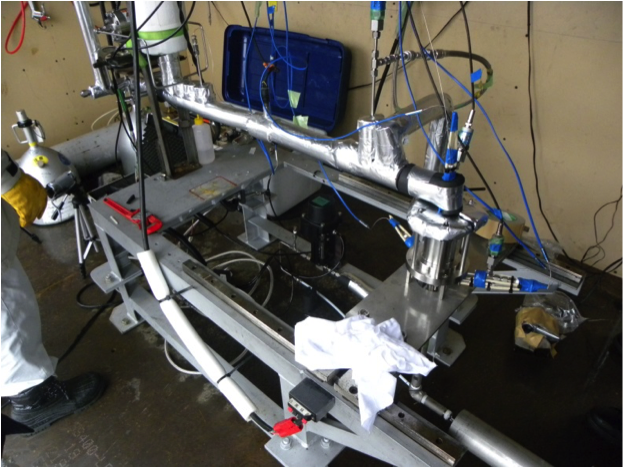
\includegraphics[width=15cm]{\FigAddTwo/LOXLinePho.png}
%\caption{LOXタンク外観}
%\label{fig:LOXTankPho}
%\end{figure}

\begin{figure}
\centering
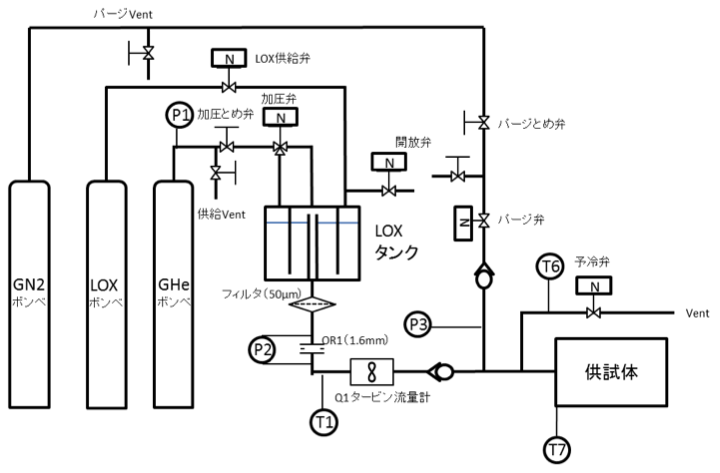
\includegraphics[width=15cm]{\FigAddTwo/LOXLine.png}
\caption{供給系系統図}
\label{fig:LOXLine}
\end{figure}

\subsection{計測系}
データロガーには、植松電機殿所有のEDX-100Aを用いた。サンプリングレートは200Hzとした。計測項目を以下に示す。
\begin{description}
\item[P1]GHe供給圧
\item[P2]オリフィス差圧
\item[P3]インジェクタ上流圧
\item[P4]プリバーナ圧
\item[P5]混合室圧
\item[Q1]LOX体積流量
\item[T1]オリフィス下流温度
\item[T2]インジェクタ上流温度
\item[T3]ノズル上流温度(内径)
\item[T4]ノズル上流温度(中心)
\item[T5]ノズル下流温度
\item[T6]予鈴温度
\item[T7]インジェクタフランジ温度
\end{description}
供試体周りの計測系の概略図を図\ref{}に、ノズル付近の内観を図\ref{fig:NozzleThermo}示す。
\\
高速度カメラによる可視化データ取得も行った。

\begin{figure}[htbp]
\begin{tabular}{cc}
\begin{minipage}{.5\textwidth}
\begin{center}
\centering
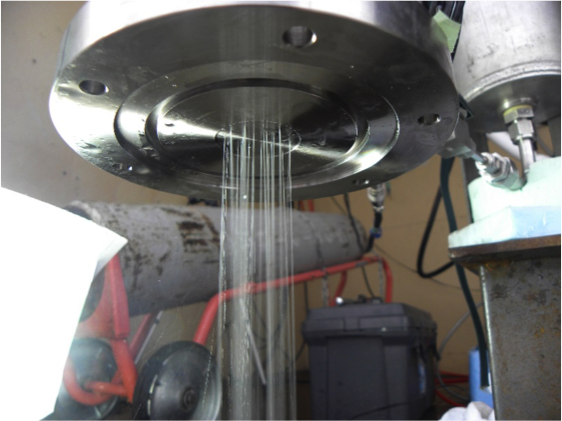
\includegraphics[width=7cm]{\FigAddTwo/Injector.png}
\caption{インジェクタ外観}
\label{fig:Injector}
\end{center}
\end{minipage}
\begin{minipage}{.5\textwidth}
\begin{center}
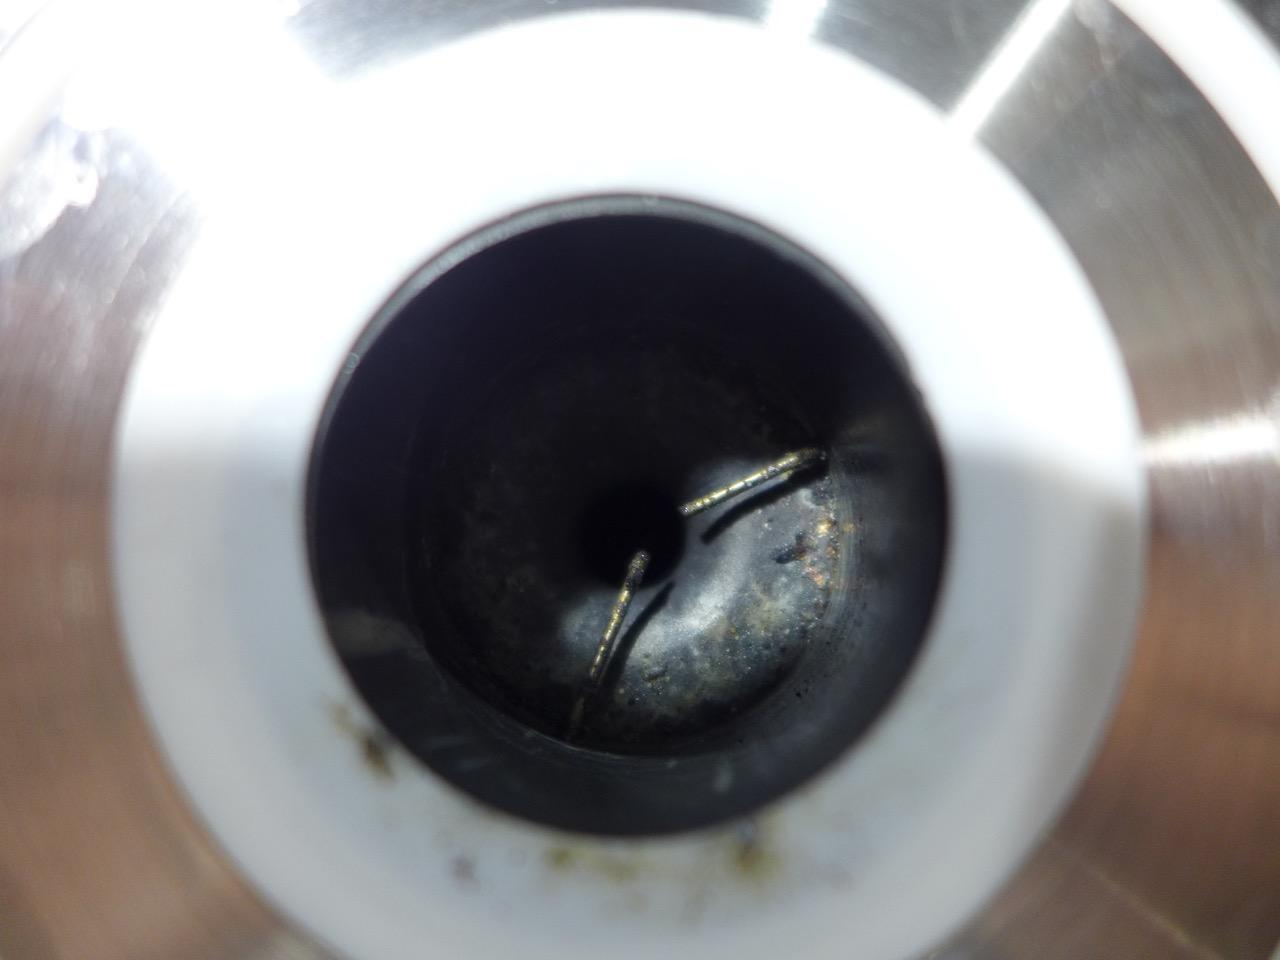
\includegraphics[width=7cm]{\FigAddTwo/NozzleThermo.jpg}
\caption{ノズル付近内観}
\label{fig:NozzleThermo}
\end{center}
\end{minipage}
\end{tabular}
\end{figure}

\subsection{制御系}
制御系は、植松電機どの所有の設備を用いた。ニクロム線加熱スイッチ、開放弁スイッチ、パージベンスイッチ、冷却弁スイッチにより構成されている。ニクロム線加熱時間、加圧弁開放時間、開放弁開はタイマーにより制御可能である。
\\
供試体1を使用した燃焼気化実験では、ニクロム線を加熱を開始した後に、LOXタンクの自己加圧によりインジェクタから放出される酸素と燃料が着火したことをビデオモニタにより確認した時に、加圧弁スイッチをオンにし、本着火を開始した。
規定の加圧弁開時間を終了したところで、加圧弁が閉じられて、開放弁が開となりLOXタンク圧力が開放される。それと同時に手動でパージ弁を開とし、窒素によるパージを行う。
供試体2を使用した燃焼気化実験では、外殻をステンレスで覆っているため、ノズル上流温度が上昇し始めたら着火したと判定し、加圧弁スイッチをオンにした。その他の手順は供試体1での実験と同様である。
ニクロム線設置位置を図\ref{fig:Nichrome}、着火判定した点を図\ref{fig:Ignition}
\begin{figure}
\centering
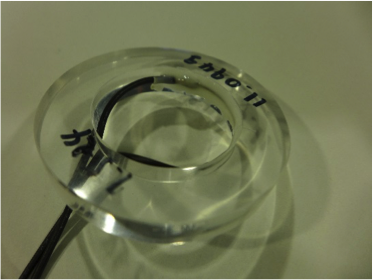
\includegraphics[width=10cm]{\FigAddTwo/Nichrome.png}
\caption{ニクロム線}
\label{fig:Nichrome}
\end{figure}
\begin{figure}
\centering
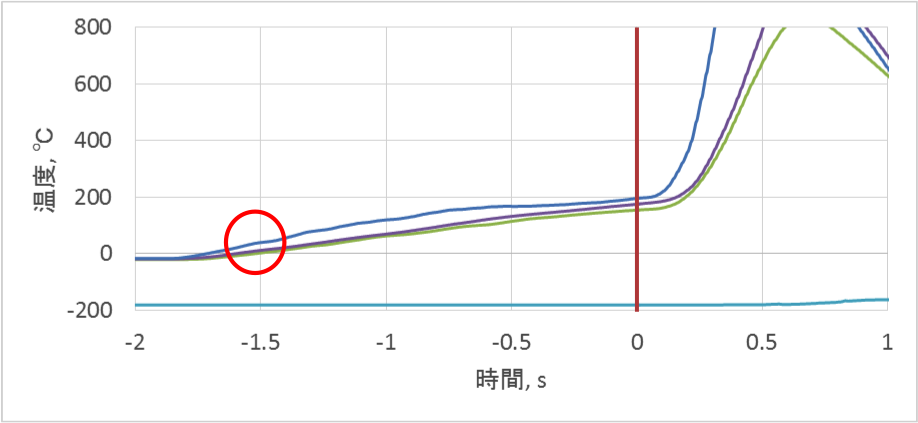
\includegraphics[width=11cm]{\FigAddTwo/Ignition.png}
\caption{着火判定した点}
\label{fig:Ignition}
\end{figure}



\section{水流し試験}
本実験では流量計測にタービン流量計の他にオリフィス差圧とインジェクタ差圧を使用した。
差圧から流量を計測するために、各差圧の流量係数を確認する必要がある。
GHe供給圧をパラメータとし、水を30秒以上流し、噴出した水の総量から、水の流量を求めた。水の噴射の様子を図に示す。
\\
流量定数はベルヌーイの定理と連続の式から導出できる。
\begin{eqnarray}
P_{1} + \frac{1}{2} \rho_{1} u^2_{1} &=& P_{2} + \frac{1}{2} \rho_{2} u^2_{2}  \nonumber \\
u^2_{2} - u^2_{1} &=& \frac{2(P_{1}-P_{2})}{\rho} 
\label{eq:vel}
\end{eqnarray}
\begin{eqnarray}
u_{1}A_{1} &=& u_{2}A_{2}  \nonumber \\
u_{2} &=& u_{1}\frac{A_{1}}{A_{2}}
\label{eq:con}
\end{eqnarray}
\ref{eq:con}を\ref{eq:vel}に代入する。
%\begin{eqnarray}
%u_{2}=\frac{1}{\sqrt{1-(\frac{A_2}{A_1})^2}} \sqrt{\frac{2(P_{1}-P_{2})}} \\
%\end{eqnarray}



\clearpage
\end{document}
